\section{收敛与计算成本}
\label{sec:newton-cost}

前四节各解决了一个困难。于是要问：在同样的精度要求下，从起点走到终点，这些方法各要花多少计算，局部收敛快是否就意味着总成本低？

\paragraph{统一的比较口径}
沿用第~\ref{chap:smooth-foundations}章的口径：所有方法以$\lVert\bm{g}^{(t)}\rVert_2\leq\varepsilon$为停止标准，返回最后的迭代点，总成本是各轮成本之和。每轮的成本分三部分：读取目标和导数、线性代数运算、线搜索的函数计算。

记一次函数、梯度、Hessian、Hessian向量积的成本为$c_f,c_g,c_H,c_{Hv}$。对稠密问题，$c_{Hv}$约为$2n^2$次运算。表~\ref{tab:newton-cost-per-iter}按每轮的成本比较各方法，并把保障分开写。

\begin{BookInlineTable}
  \centering
  \small
  \begin{tabular}{@{}llll@{}}
    \toprule
    方法 & 每轮主要成本 & 远处的保障 & 近解行为 \\
    \midrule
    Newton法 & $c_H$，分解$\tfrac13n^3$ & 无 & 二次 \\
    阻尼Newton & 上述加回溯的$c_f$ & 正定时下降 & 接受整步后二次 \\
    对角平移 & $c_H$，分解可能重复若干次 & $\bm{g}\to\bm{0}$ & 修正消失后二次 \\
    谱修正 & $c_H$，特征分解 & $\bm{g}\to\bm{0}$ & 修正消失后二次 \\
    修正Cholesky & $c_H$，分解约$\tfrac13n^3$ & $\bm{g}\to\bm{0}$ & 修正消失后二次 \\
    Newton-CG & $k_tc_{Hv}$，无分解 & 方向下降，回溯 & 由$\eta_t$决定 \\
    \bottomrule
  \end{tabular}
  \caption{各方法单轮成本和收敛保障的比较，$k_t$是第$t$轮内层的Hessian向量积次数。“$\bm{g}\to\bm{0}$”需要定理~\ref{thm:newton-modified-global}的条件，“修正消失”要求解处Hessian正定且修正规则先试零修正。}
  \label{tab:newton-cost-per-iter}
\end{BookInlineTable}

\paragraph{两个阶段分开计算}
定理~\ref{thm:newton-damped-global}和定理~\ref{thm:newton-unit-step}给出阻尼Newton法的总步数上界。取强凸常数$\mu$、光滑常数$L$、Hessian的Lipschitz常数$M$和定理中的阈值$\tau$。

第一阶段是$\lVert\bm{g}^{(t)}\rVert_2>\tau$的轮次。由定理~\ref{thm:newton-damped-global}证明的第四步，每轮目标至少下降
\[
 \gamma=\frac{c\beta\tau^2}{\kappa L}.
\]
目标总下降量不超过$f(\bm{x}^{(0)})-f^\star$，所以这一阶段的轮数不超过$(f(\bm{x}^{(0)})-f^\star)/\gamma$。

第二阶段记$b_t=M\lVert\bm{g}^{(t)}\rVert_2/(2\mu^2)$，由式~\eqref{eq:newton-gradient-quadratic}，$b_{t+1}\leq b_t^2$，且起始时$b\leq\tfrac12$。要使$\lVert\bm{g}\rVert_2\leq\varepsilon$，只需$2^{-2^t}\leq M\varepsilon/(2\mu^2)$。于是总步数满足
\begin{equation}
 T\leq\frac{f(\bm{x}^{(0)})-f^\star}{\gamma}+\Bigl\lceil\log_2\log_2\frac{2\mu^2}{M\varepsilon}\Bigr\rceil.
 \label{eq:newton-total-iterations}
\end{equation}

第二项随精度增长极慢：$\varepsilon$从$10^{-6}$收紧到$10^{-12}$，只多大约一步。第一项与$\varepsilon$无关，却含有问题常数，通常主导总步数。所以局部收敛阶回答“到了解附近以后怎样”，全局成本回答“总共要花多少”，只看前者不足以判断整体效率。

\paragraph{贵的一步和便宜的很多步}
Newton法每轮贵，轮数少；一阶方法每轮便宜，轮数多。若梯度下降需要$T_{\mathrm{GD}}$轮，Newton法需要$T_{\mathrm{N}}$轮，分解成本记为$c_{\mathrm{fac}}$，则Newton法更划算的条件是
\begin{equation}
 T_{\mathrm{N}}\bigl(c_g+c_H+c_{\mathrm{fac}}\bigr)<T_{\mathrm{GD}}\,c_g.
 \label{eq:newton-breakeven}
\end{equation}

主例从$(\tfrac12,0)$出发，把梯度范数降到$10^{-6}$，回溯梯度下降用了$245$轮、$792$次函数计算，Newton法用了$5$轮。二维问题的分解几乎不花时间，所以Newton法的总成本低得多。

规模变大，结论就可能相反。取稠密$n=10^4$，一次Cholesky分解约$3.3\times10^{11}$次运算，一次梯度若与$n^2$同量级，一次分解约相当于$1700$次矩阵向量乘积。若不到一千次梯度步就能达到要求的精度，Newton法在稠密实现下就不划算。反过来，Hessian稀疏时分解可能很便宜，三对角矩阵的分解只需$O(n)$次运算。比较时必须用实际的结构，不能只看$n$。

\paragraph{内层的精度也要计入成本}
非精确方法的比较要把内层计入。取式~\eqref{eq:newton-running-objective}的链式推广，$n=1000$：
\begin{equation}
 f(\bm{x})=\sum_{i=1}^{n-1}\Bigl[\frac12(x_i-1)^2+(x_{i+1}-x_i^2)^2\Bigr].
 \label{eq:newton-chain-objective}
\end{equation}
从分量交替取$-1.2$和$1$的点出发，用带回溯（$c=10^{-4}$）的Newton-CG，把梯度范数降到$10^{-9}$。结果列在表~\ref{tab:newton-cg-cost}中，图~\ref{fig:newton-cost}画出了全过程。

\begin{BookInlineTable}
  \centering
  \begin{tabular}{@{}lcc@{}}
    \toprule
    误差比例 & 外层轮数 & $\bm{H}\bm{v}$总次数 \\
    \midrule
    $\eta=0.5$ & $29$ & $93$ \\
    $\eta=0.1$ & $15$ & $72$ \\
    $\eta_t=\min\{0.5,\sqrt{\lVert\bm{g}^{(t)}\rVert_2}\}$ & $17$ & $100$ \\
    $\eta=10^{-10}$（近乎精确求解） & $12$ & $357$ \\
    \bottomrule
  \end{tabular}
  \caption{目标~\eqref{eq:newton-chain-objective}上不同误差比例的成本。内层解得越精确，外层轮数越少，总乘积次数却可能大幅增加。}
  \label{tab:newton-cg-cost}
\end{BookInlineTable}

\begin{BookInlineFigure}
  \centering
  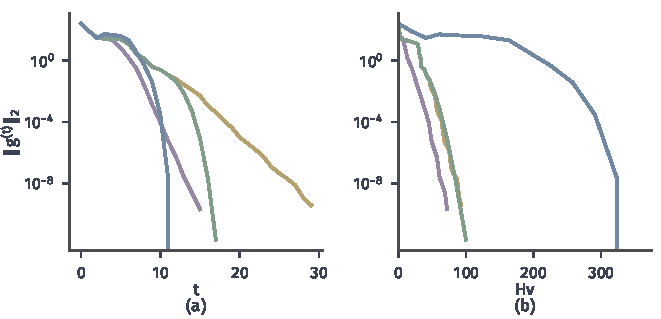
\includegraphics[width=112mm]{figures/05-optimization/02-smooth-optimization/matplotlib/newton-cost/figure.pdf}
  \caption{目标~\eqref{eq:newton-chain-objective}上Newton-CG的进展，$n=1000$。(a)梯度范数随外层轮数$t$的变化，(b)随累计Hessian向量积次数的变化。黄线$\eta=0.5$，紫线$\eta=0.1$，绿线$\eta_t=\min\{0.5,\sqrt{\lVert\bm{g}^{(t)}\rVert_2}\}$，蓝线$\eta=10^{-10}$。蓝线在(a)中外层轮数最少，在(b)中总成本最高。}
  \label{fig:newton-cost}
\end{BookInlineFigure}

这组数据说明两点。第一，把内层解到接近精确，与$\eta=0.1$相比外层只少了三轮，乘积次数却是它的五倍。第二，表中自适应规则的乘积次数并不最少，$\eta=0.1$在这个例子上反而更好。自适应规则的好处是不需要调参并且保证局部快速收敛，而不是在每个问题上都最省。

还要注意目标~\eqref{eq:newton-chain-objective}的Hessian是三对角的，稀疏Cholesky分解每次只要$O(n)$次运算，这种情况下精确Newton法也相当便宜。Newton-CG的优势主要在Hessian稠密、结构不便分解、或者根本不想形成矩阵的时候。

\paragraph{三种手段的组合}
阻尼、修正、非精确求解作用在迭代的不同环节，可以按需要组合。实际程序中常见的组合是：Hessian可以分解时，用试探$\delta$的修正Cholesky或对角平移加回溯；规模太大时，用Newton-CG加回溯，负曲率时截断。每一种组合的保证都要对应地核对：下降方向由哪一环保证，步长由哪一环保证，局部速度又由哪些量趋于零来保证。
